%\documentclass[10pt,twocolumn]{article}
\documentclass[10pt]{article}

\usepackage{times}
\usepackage{color}
\usepackage{graphicx}
\usepackage[hidelinks]{hyperref}
\usepackage{xspace}
\usepackage{setspace}
\usepackage{fullpage}
\usepackage{subcaption}
\usepackage{pbox}

\definecolor{CBlue}{rgb}{0.33,0.63,0.83}
%\newcommand{\david}[1]{}
%\newcommand{\shaddi}[1]{}
%\newcommand{\omer}[1]{}

\newcommand{\david}[1]{[\textcolor{red}{\textit{David: #1}}]}
\newcommand{\shaddi}[1]{[\textcolor{CBlue}{\textit{Shaddi: #1}}]}
\newcommand{\omer}[1]{[\textcolor{green}{\textit{Omer: #1}}]}

\title{Classifying Runtime Performance with SVM}

\author{David Eliahu \and Shaddi Hasan \and Omer Spillinger}

\begin{document}

\maketitle

\begin{abstract}
    We present a machine-learning based technique for the problem of \emph{algorithm selection}, specifically focusing on algorithms for dense matrix multiplication (DMM).
    Dense matrix multiplication is a core part of many high-performance computing and machine learning algorithms, but the performance of DMM algorithms can vary significantly based on their input and the performance characteristics of each particular machine.
    We model machine performance using support vector machines and show that only a small sample of possible inputs is sufficient to determine the best choice of algorithm over a wide range of possible inputs and even over different machines (by training a model per machine).
    We find that by using this classifier-based approach and choosing the best algorithm to use at runtime, we are able to achieve at least a 0.5\% and as much as a 28\% increase in performance over choosing a single algorithm a priori.
\end{abstract}

\section{Introduction}
Computer scientists develop algorithms---it's just what we do, we can't help it.
Algorithm designers produce an ever-increasingly set of techniques for solving an ever-wider set of problems.
Indeed, algorithm selection itself has become a challenging problem, particularly in fields where performance is critical such as high-performance computing and machine learning.
The factors that influence algorithm performance are extremely complicated, and understanding how an algorithm will perform given an input and a particular machine can require extensive domain knowledge.
Performance can even vary significantly from system to system due to differences in factors such as memory hierarchy, machine architecture, utilization, and so on.
This problem is even more pronounced on virtualized infrastructure: the application developer really has no way of knowing how the underlying hardware will perform, or even if her application will always be running on the same hardware (e.g., due to virtual machine migration).

All this made us ask ourselves, how can we \emph{predict} the optimal algorithm to use in a given situation?
Being able to do so would be a significant benefit to developers: such a technique could be incorporated into libraries so that developers could write software oblivious of the underlying algorithmic implementation, confident that the library would choose the proper algorithm.

One solution to this problem would be to develop a model of machine performance and analytically determine the best algorithm to use for a given input.
Clearly, this approach wouldn't scale---the model would be enormously complex, and would need to be developed for every combination of machine and algorithm.

One could also take an empirical approach: simply measure how algorithms perform on a given machine under different inputs.
A na\"{\i}ve solution would be to exhaustively search the space of possible inputs; this is intractable in the general case, and even in situations where the range of possible inputs is finite exhaustive search is time consuming.

The complexity of performance classification lends itself to a machine learning approach.
Rather than building a complex model of machine performance, we can train a classifier on a set of training examples to estimate the best algorithm to use.
In contrast to exhaustive search, a classifier-based approach need not explore a large portion of the search space.
The user can make an explicit tradeoff between classifier accuracy and training time.

We take this classifier-based approach in our project.
In this work, we focus on dense matrix multiplication (DMM).
We chose this problem for several reasons.
First, DMM is an important step in many HPC and machine learning tasks, and it often represents the computational performance bottleneck for those tasks.
Thus, even relatively small performance gains for DMM can translate to real savings for large tasks.
Secondly, a plethora of algorithms for DMM exist in the literature.
Two of the authors have developed a communication-avoiding algorithm for DMM called CARMA; CARMA's approach is substantially different than the industry-standard algorithm MKL, making it likely that it would have different performance properties.
Finally, DMM is easily parameterizable---in general, performance is dictated by the dimensions of the input matrices.

We perform classification using a support vector machine.
We evaluate our classifier on a set of multiplications of matrices ranging in size from 64 x 64 to 3250 x 3250---a state space of over 32 billion possible inputs.
We find that our classifier achieves good results across multiple machines, with F1 scores ranging from 0.75 to 0.88, and that training on only a few hundred points is sufficient to achieve this level of accuracy.
Finally, using our approach we observe performance increases of up to 28\% versus choosing an algorithm a priori.

The remainder of the paper is organized as follows.
We first discuss our dataset and its generation.
We then describe our approach towards evaluation and analysis.
In section~\ref{s:eval} we describe our results before considering future directions and concluding.

\section{Related Work}
\label{s:related}
Cite some stuff.

\section{Data}
Our project takes an empirical approach to the algorithm selection problem.
Thus, our first step is to collect data for analysis.

\subsection{Generating Data}
We featurize matrix multiplications based on the dimensions of the input matrices: M, K, and N.
These features represent the size of each dimension of a matrix multiplication of the form $M\times{K} * K\times{N}$.
We generated random dense matrices with real-valued floating point numbers ranging in size from $64\times{64}$ to $3250\times{3250}$.
We varied each dimension in evenly-spaced increments across that range.\shaddi{David, you should add more detail about this}.
Note that this means we generated a range of rectangular matrices, not just square ones.

This step results in 1000 possible matrix multiplications (i.e., combinations of M, K, and N).
We then run each of these matrix multiplications using both of our algorithms under test (MKL and CARMA) and record the performance of each multiplication in gigaflops/second.
We repeat each multiplication three times and compare the mean performance for each algorithm.
This constitutes a single datapoint for our classifier: a tuple (M,K,N) and a binary label of which algorithm performed better.
Finally, we performed this process on three separate machines with different architectures, for a total of 18,000 matrix multiplications and 3,000 data points.
The machines we used are shown in Table~\ref{t:machines}.

\shaddi{Maybe say something about the tools we used to generate and run the experiments?}

\begin{table}[t]
    \begin{center}
        \begin{tabular}{c|c|c|c}
            Machine & Cores & CPU Type & Memory \\ \hline
            Emerald & 32 & Intel Xeon X7560 & 128GB \\
            Hopper & 24 & AMD ``MagnyCours'' & 32GB \\
            Sandy & 8 & Intel i7-2600 & 16GB \\
        \end{tabular}
    \end{center}
    \caption{Machines used for evaluation.}
    \label{t:machines}
\end{table}

\subsection{Limitations}
Our data has a few limitations.
First and foremost, our largest matrix is $3250\times{3250}$.
While this is a large matrix, it still fit in memory on all our machines; we did not explore extremely large matrix sizes, though we believe our technique is general enough to scale to those as well.
Secondly, some of the machines we used to generate data were shared machines.
As a result, our performance would sometimes fluctuate significantly between runs; we considered average performance to account for this, but due to time constraints we were only able to consider an average of three runs.
Nevertheless, our classification results were strong, so we do not believe that the noise introduced by this significantly impacted our evaluation.

\section{Classification}
\label{s:class}
Intuitively, we expected the regions in which each algorithm performed better to be highly nonlinear.
As a result, we chose to use a support vector machine for classification, as these are known to have good performance for nonlinear classification.
Specifically, we used MATLAB's~\shaddi{cite} implementation of SVM.
We chose to compare two kernels, the Gaussian radial basis function (RBF) and the multilayer perceptron (MLP).

As described in section~\ref{s:data:gen}, we featurized DMM by using the sizes of the input matrices: M, K, and N.
The output of our classifier was the algorithm that performed better for a given tuple (M, K, N).
The classifier only considered the binary training data---we did not take into account how much better an algorithm performed at each point; we leave this weighted classification to future work.

\subsection{Training}
We trained our classifier on each of our three testing machines.
Our results, shown in Figure~\ref{fig:training}, were surprising.
While we expected some machine-to-machine variation, the regions where each algorithm performs better are substantially different across machines.
Indeed, Emerald and Sandy have diametrically opposed training results.
\shaddi{Wasn't there a reason for this that you all mentioned? Would be cool to add it.}
This is a key result: approaches that do not consider per-machine variation are certain to use the wrong algorithm in many cases.
We also note that the regions of optimal performance for each algorithm are in fact nonlinear.

\begin{figure*}[t]
    \centering
        \begin{subfigure}[t]{0.33\textwidth}
            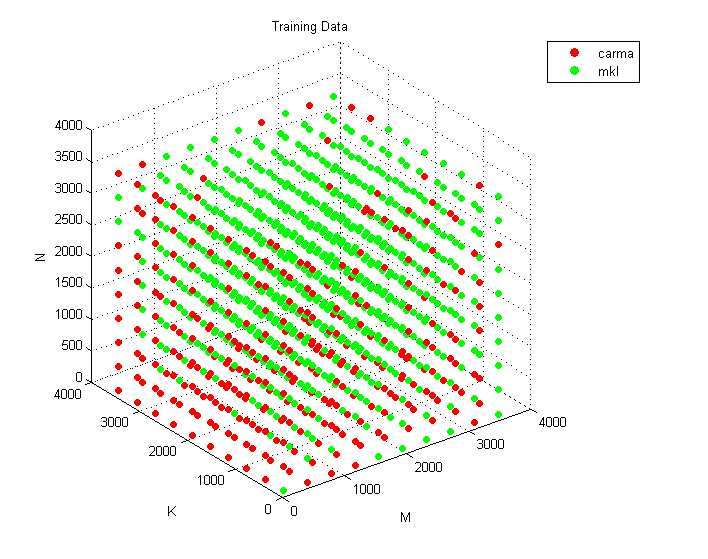
\includegraphics[width=\textwidth]{figures/emerald_train.png}
            \caption{Emerald}
            \label{f:train_emerald}
            \end{subfigure}
        \begin{subfigure}[t]{0.33\textwidth}
            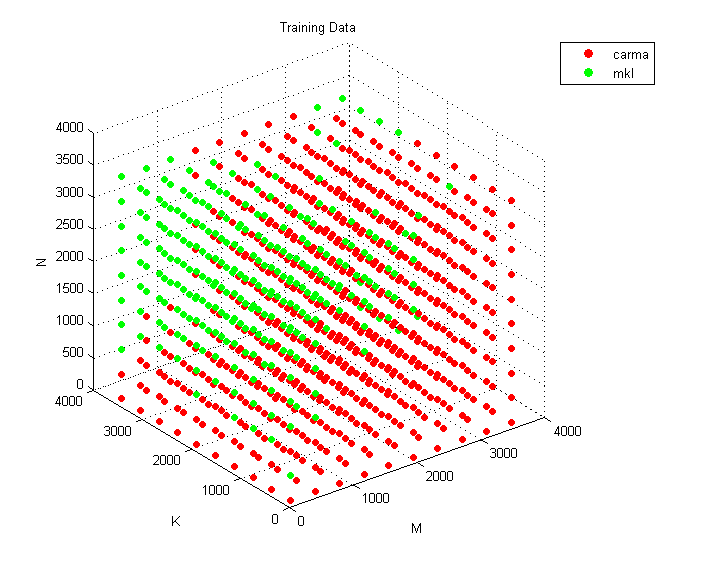
\includegraphics[width=\textwidth]{figures/hopper_train.png}
            \caption{Hopper}
            \label{f:train_hopper}
        \end{subfigure}
        \begin{subfigure}[t]{0.33\textwidth}
            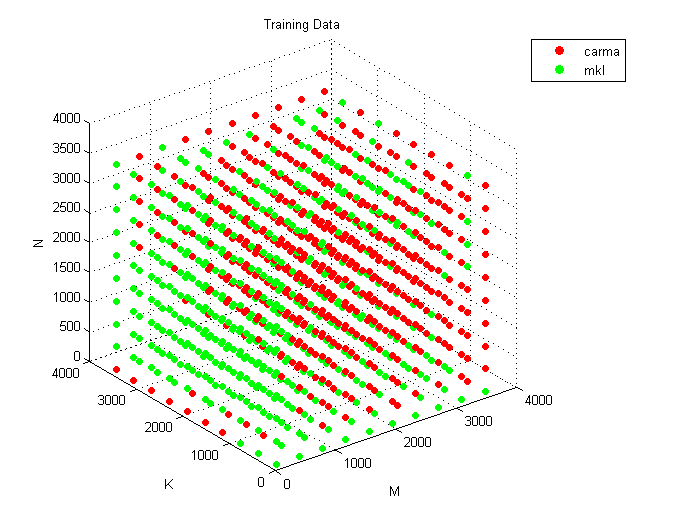
\includegraphics[width=\textwidth]{figures/sandy_train.png}
            \caption{Sandy}
            \label{f:train_sandy}
        \end{subfigure}
        \caption{Training results for each of our three machines. Green dots represent datapoints where MKL outperformed CARMA, red dots indicate the reverse. Note how the results are almost completely reversed for Emerald and Sandy.}
    \label{fig:training}
\end{figure*}

Another surprising result of our training was the fact that CARMA performed well for such large regions.
The developers of that algorithm had designed it for multiplication of ``long, skinny'' matrices, and it outperformed MKL for those on all three of our machines.
However, its strong performance for other types of matrices was unexpected.
This is likely to do with... \shaddi{something?}.

\subsection{Classifying}
In order to evaluate our classifier, we needed to generate random datapoints for testing.
We randomly generated values for M, K, and N within our training space, and and duplicated our data-collecting procedure to time the multiplications and record which algorithm ran faster.
After gathering this test data, we removed the true class labels and ran the values for M, K, and N through our classifier (once per machine for each kernel).
Given the true and predicted label for each testing datapoint, we now had enough information to evaluate our classifier.
See Figure~\ref{fig:classifying} for the results of this procedure.

\begin{figure*}[t]
    \centering
        \begin{subfigure}[t]{0.33\textwidth}
            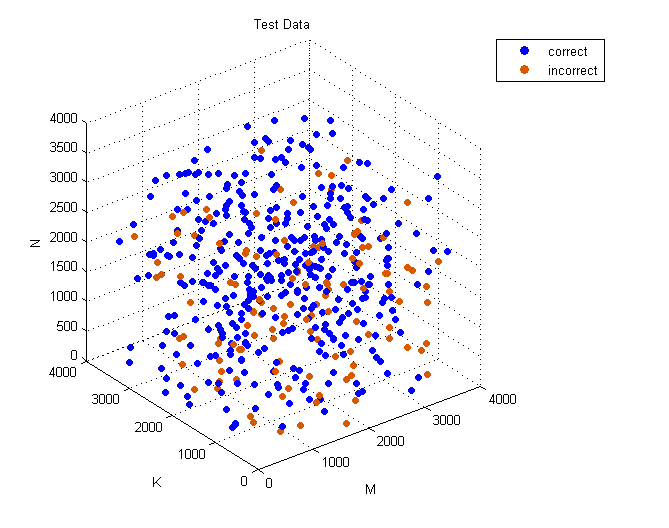
\includegraphics[width=\textwidth]{figures/emerald_test_rbf.png}
            \caption{Emerald - RBF}
            \label{f:classify_rbf_emerald}
        \end{subfigure}
        \begin{subfigure}[t]{0.33\textwidth}
            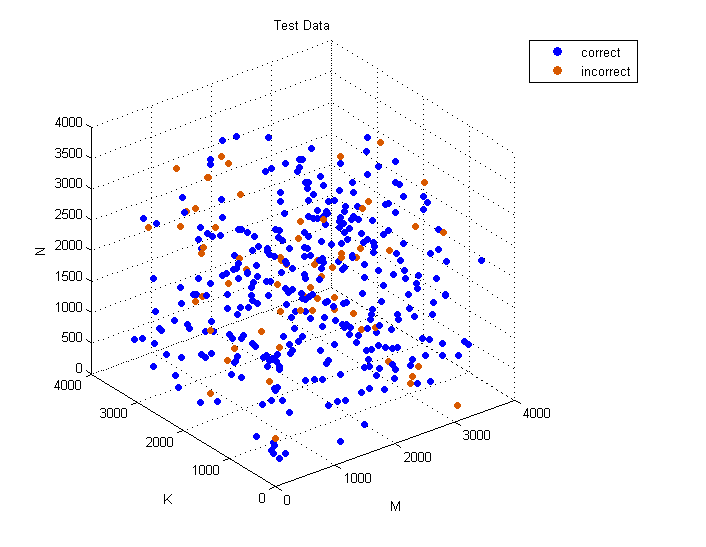
\includegraphics[width=\textwidth]{figures/hopper_test_rbf.png}
            \caption{Hopper - RBF}
            \label{f:classify_rbf_hopper}
        \end{subfigure}
        \begin{subfigure}[t]{0.33\textwidth}
            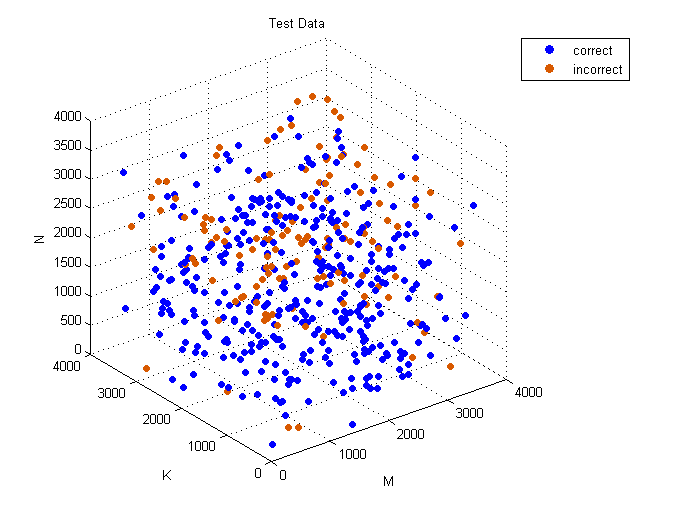
\includegraphics[width=\textwidth]{figures/sandy_test_rbf.png}
            \caption{Sandy - RBF}
            \label{f:classify_rbf_sandy}
        \end{subfigure}
    \centering
        \begin{subfigure}[t]{0.33\textwidth}
            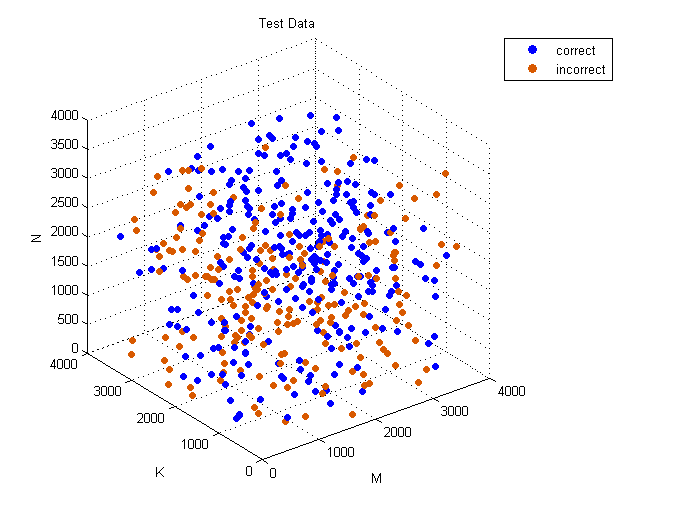
\includegraphics[width=\textwidth]{figures/emerald_test_mlp.png}
            \caption{Emerald - MLP}
            \label{f:classify_mlp_emerald}
        \end{subfigure}
        \begin{subfigure}[t]{0.33\textwidth}
            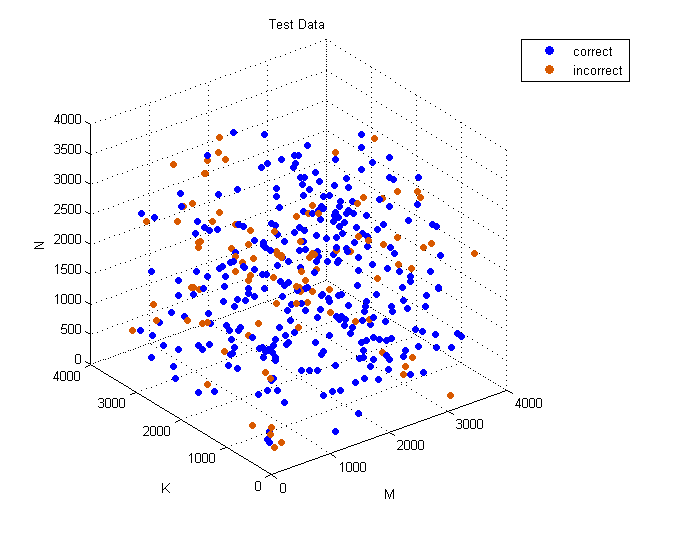
\includegraphics[width=\textwidth]{figures/hopper_test_mlp.png}
            \caption{Hopper - MLP}
            \label{f:classify_mlp_hopper}
        \end{subfigure}
        \begin{subfigure}[t]{0.33\textwidth}
            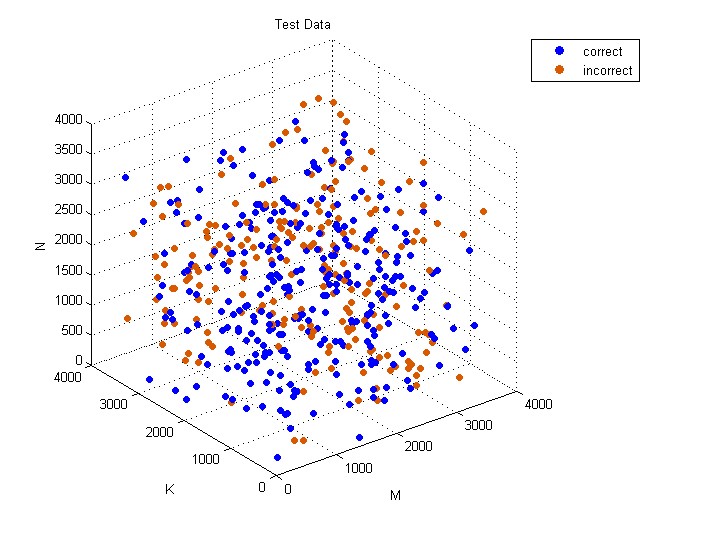
\includegraphics[width=\textwidth]{figures/sandy_test_mlp.png}
            \caption{Sandy - MLP}
            \label{f:classify_mlp_sandy}
        \end{subfigure}
        
        \caption{Testing results for each of our three machines, for each kernel (RBF and MLP). Blue dots represent datapoints where our classifier correctly predicted which algorithm was faster, and orange dots represent incorrect classifications. Note that the RBF kernel outperforms the MLP kernel on all machines (most significantly on Emerald and Sandy)}
    \label{fig:classifying}
\end{figure*}

It is worth noting that the majority of incorrect classifications occur on or near the decision boundaries our classifier has generated.
This is due to the fact that along these decision boundaries, the performance of MKL and CARMA is comparable.
On any given trial, CARMA may slightly outperform MKL, or MKL may marginally beat CARMA.
Therefore, the class that our classifier assigns to datapoints along a decision boundary may not match the given instance of performance data that we gathered, even though the actual performance difference is relatively minor.

To better visualize this phenomenon, we simplified the problem by reducing it to a two-dimensional classification problem.
By only considering datapoints where K = N, we were able to train a 2D classifier to better visualize the decision boundary.
See Figure~\ref{fig:2D}.

\begin{figure*}[t]
    \centering
        \begin{subfigure}[t]{0.49\textwidth}
            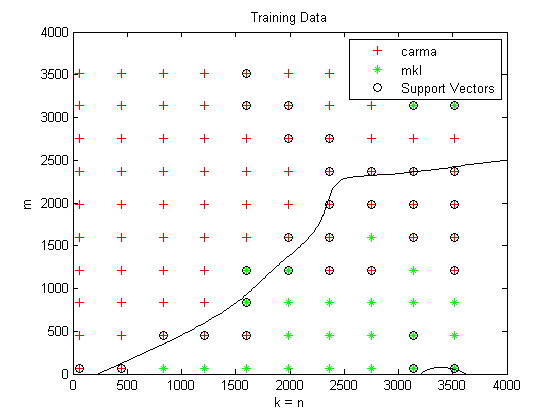
\includegraphics[width=\textwidth]{figures/hopper2D_train_mlp.png}
            \caption{Training: Green dots represent datapoints where MKL outperformed CARMA, red dots indicate the reverse.}
            \label{f:train_hopper_2D}
            \end{subfigure}
        \begin{subfigure}[t]{0.49\textwidth}
            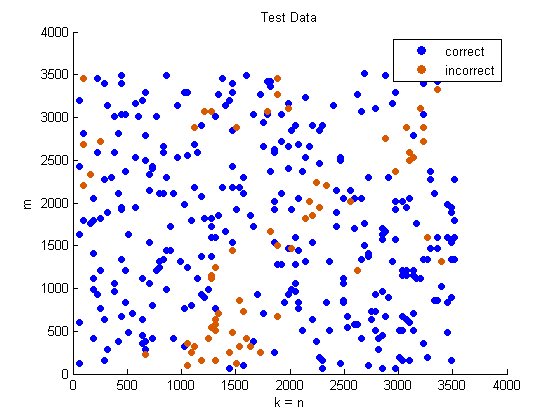
\includegraphics[width=\textwidth]{figures/hopper2D_test_mlp.png}
            \caption{Testing: Blue dots represent datapoints where our classifier correctly predicted which algorithm was faster, and orange dots represent incorrect classifications.}
            \label{f:test_hopper_2D}
        \end{subfigure}
        \caption{Training vs. testing on Hopper using the MLP kernel. Observe that the majority of incorrect classifications (orange dots in subfigure b) occur along the decision boundary, where CARMA and MKL exhibit similar performance behavior.}
    \label{fig:2D}
\end{figure*}

On average, the performance loss resulting from an incorrect classification is only 9.6\%, supporting the observation that the majority of these misclassifications occur along decision boundaries where CARMA's and MKL's performance are comparable.

\section{Evaluation}
\label{s:evaluation}


We evaluate the performance of our classifier using F1 scores (see Table~\ref{t:F1_scores}).
In summary, our classifier performs best on Hopper, which yields an F1 score of 0.88 (with the RBF kernel).
Our classifier performs worst on Sandy, on which it achieves an F1 score of 0.75 (also using the RBF kernel).
On all three machines, the RBF kernel outperforms the MLP kernel.

\begin{table}[t]
    \begin{center}
        \begin{tabular}{c|c|c}
            Machine & RBF Kernel & MLP Kernel \\ \hline
            Emerald & 0.82 & 0.64 \\
            Hopper & 0.88 & 0.82 \\
            Sandy & 0.75 & 0.59 \\
        \end{tabular}
    \end{center}
    \caption{F1 scores for each machine and kernel. Note that on all machines, the RBF kernel outperformed the MLP kernel.}
    \label{t:F1_scores}
\end{table}

In order to measure how many datapoints are required to train an accurate classifier, we explored the effects of reducing the size of our training set.
In this experiment, we randomly selected X\% of our original 1000 training points, for X ranging from 1\% to 100\%.
After training our classifier with this random X\% of training data, we measured the resulting F1 score on the test data. See Figure~\ref{fig:convergence}.

\begin{figure*}[t]
    \centering
        \begin{subfigure}[t]{0.33\textwidth}
            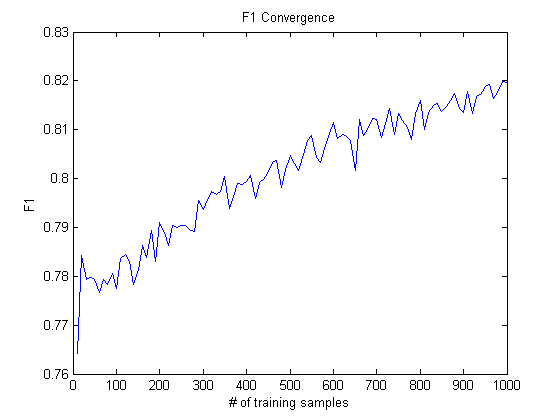
\includegraphics[width=\textwidth]{figures/F1_convergence_emerald.png}
            \caption{Emerald}
            \label{f:F1_emerald}
            \end{subfigure}
        \begin{subfigure}[t]{0.33\textwidth}
            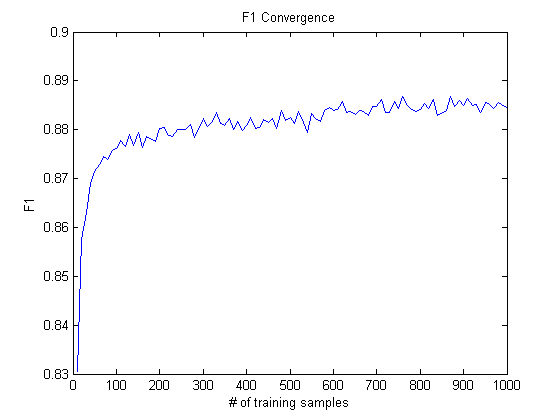
\includegraphics[width=\textwidth]{figures/F1_convergence_hopper.png}
            \caption{Hopper}
            \label{f:F1_hopper}
        \end{subfigure}
        \begin{subfigure}[t]{0.33\textwidth}
            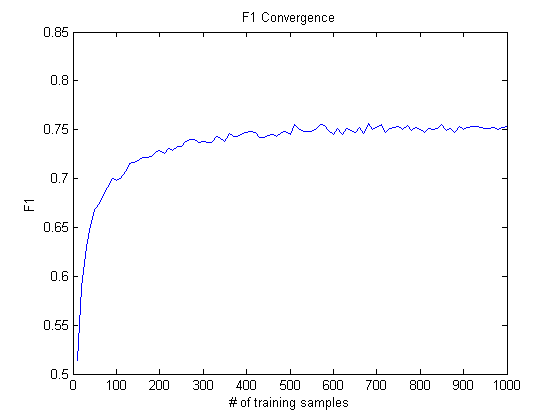
\includegraphics[width=\textwidth]{figures/F1_convergence_sandy.png}
            \caption{Sandy}
            \label{f:F1_sandy}
        \end{subfigure}
        \caption{F1 convergence on each machine (using the RBF kernel). Sandy and Hopper require fewer than 500 datapoints to generate accurate performance models, while Emerald requires more than 1000 (due to Emerald's more complicated performance patterns).}
    \label{fig:convergence}
\end{figure*}

Of course, the number of training points required to build an accurate model will vary widely by machine and algorithm.
As shown in Figure~\ref{fig:convergence}, although Sandy and Hopper require fewer than 500 datapoints to achieve a maximal F1 score, Emerald requires more than 1000.
This is due to the fact that performance patterns on Emerald are more complex.
We don't have a theoretical model to understand this complexity, further validating the value our empirical approach.

We also performed tests to quantify the benefit of using our algorithm selection technique.
How much do we gain by using our classifier to select the optimal algorithm?
It depends on the machine, as well as what algorithm would have been chosen otherwise.
For example, using our classifier on Emerald yields an 11.3\% average speedup over using only CARMA, and a 5.7\% speedup over using just MKL (this includes the penalties of misclassifications).
On Hopper, our classifier enjoys a healthy 28.0\% gain over using MKL only.
For complete results, see Table~\ref{t:improvements}.

\begin{table}[t]
    \begin{center}
        \begin{tabular}{c|c|c}
            Machine & Selection vs CARMA Only & Selection vs MKL Only \\ \hline
            Emerald & 11.3\% & 5.7\% \\
            Hopper & 2.2\% & 28.0\% \\
            Sandy & 4.4\% & 0.9\% \\
        \end{tabular}
    \end{center}
    \caption{F1 scores for each machine and kernel. Note that on all machines, the RBF kernel outperformed the MLP kernel.}
    \label{t:improvements}
\end{table}

\section{Future Work}
\label{s:future}

The input used to train the SVM was binary: if CARMA's performance was superior to MKL's performance for a given set of matrix dimensions, the datapoint was given with the CARMA label (and vice versa for MKL).
We aim to explore techniques that account for the magnitude of the difference between the two algorithms' performances.
In other words, datapoints for which one algorithm was significantly faster should be weighted more heavily in our performance model.
Performance gains achieved by correctly selecting the faster algorithm are a more important metric for this work than a high overall classification accuracy.

In this project, we examined dense matrix multiplication on three different shared-memory machines.
However, the approach of using SVM to partition a feature space based on algorithm performance patterns can be generalized to a wide variety of other algorithms and architectures.
We aim to evaluate additional linear algebra algorithms such as QR decomposition and sparse matrix multiplication.
Furthermore, we are interested in gathering data on distributed-memory machines in which higher communication costs magnify the performance gains that can be achieved by communication-avoiding algorithms such as CARMA.

Finally, algorithm selection could be incorporated into machine learning as well as scientific computing frameworks.
After gathering sufficient training data, the framework could select the optimal algorithm for a given set of input parameters at runtime.
The number of samples required for convergence in the dense matrix multiplication case that we explored is orders of magnitude smaller than the size of the feature space (Figure~/ref{fig:convergence}).
The framework would only classify input parameters above a certain threshold because the overhead of classification cannot be justified for all cases.

\section{Conclusion}
\label{s:conclusion}
In this project, we've tackled the problem of algorithm selection for HPC and machine learning problems, specifically focusing on dense matrix multiplication.
This problem is challenging due to the complexity of analyzing machine performance a priori and due to per-machine variation in algorithm performance, the latter of which was dramatically reflected in our training results.
We found that using a support vector machine to classify the space of inputs between multiple choices of algorithms can yield good results, with F1 scores as high as 0.88 on one of our testing machines.
Moreover, achieving that level of accuracy requires a small training set---only a few hundred data points.

We believe this technique has promise for improving the performance of real applications.
The status quo requires developers to think carefully about the machines and data their applications will use, analyze the expected performance, and then choose their algorithm appropriately, hoping they've made the right choice for all time.
This need not be the case: we've demonstrated that our approach is feasible and in general improves performance over the status quo, with up to 28\% increase in performance in the best case.


\bibliographystyle{ieeetr}
\bibliography{main}

\end{document}
